\documentclass{article}

\usepackage[letterpaper,
	left=1.5in,
	right=1in,
	top=1in,
	bottom=1in,
	footskip=.25in]{geometry}
\usepackage{tikz}
\usepackage{gensymb}
\usepackage{amsmath}
\usepackage{cancel}
\usepackage{xcolor}
\usepackage{amssymb}
\usepackage{graphicx}
\usepackage{systeme}
\usepackage{hyperref}
\usepackage{pgfplotstable,filecontents}
\pgfplotsset{compat=1.9}
\usepackage[scaled=0.9]{DejaVuSansMono}
\usepackage{listings}


\renewcommand{\thefootnote}{\fnsymbol{footnote}}

\definecolor{codegreen}{rgb}{0,0.6,0}
\definecolor{codegray}{rgb}{0.5,0.5,0.5}
\definecolor{codepurple}{rgb}{0.58,0,0.82}
\definecolor{backcolour}{rgb}{0.95,0.95,0.92}

\renewcommand{\rmdefault}{ptm}

\lstdefinestyle{mystyle}{
			backgroundcolor=\color{backcolour},   
			commentstyle=\color{codegreen},
			keywordstyle=\color{magenta},
			numberstyle=\tiny\color{codegray},
			stringstyle=\color{codepurple},
			basicstyle=\ttfamily\scriptsize,
			breakatwhitespace=false,         
			breaklines=true,                 
			captionpos=b,                    
			keepspaces=true,                 
			numbers=left,                    
			numbersep=5pt,                  
			showspaces=false,                
			showstringspaces=false,
			showtabs=false,                  
			tabsize=4
		}
\lstset{style=mystyle}



\begin{document}    

\section{Materials}

to be filled

\section{Methods}
\subsection*{Device engineering}

to be filled

\subsection*{RFID-based lock system algorithm}

The locking system follows the algorithm depicted in the Figure below. It was programmed using its native \texttt{adruino} programming language. 

\begin{figure}[h!]
    \centering
    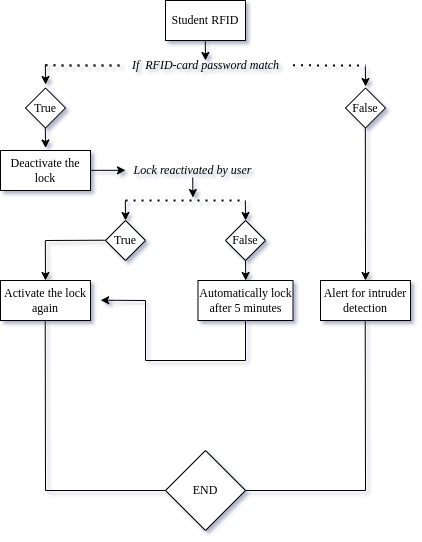
\includegraphics[width=0.7\textwidth]{fig2.png}
    \caption{Algorithm of RFID-based lock.} \label{fig:2}
\end{figure}

\subsection*{RFID-based attendance algorithm}

The main algorithm as shown in the Figure below, of the system will be written in \texttt{Python -v 3.9.1} with the student database stored offline in JavaScript Object Notation (JSON) file.

\begin{figure}[h!]
    \centering
    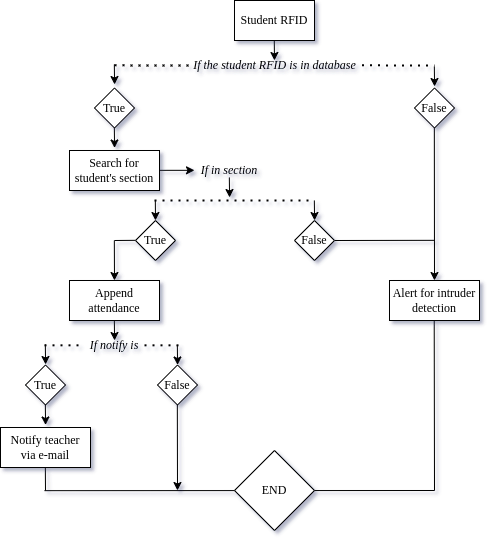
\includegraphics[width=0.7\textwidth]{fig1.png}
    \caption{Algorithm of RFID-based Attendance.} \label{fig:1}
\end{figure}

There are various third party modules used to aid the python standard library was for successful execution of the function. \texttt{pandas.DataFrame} was used for attendance of the students, as well as \texttt{pandas.to\_excel} function for everyday reporting to teachers. The email was sent using \texttt{Python}'s \texttt{smtplib} and \texttt{ssl}, Simple Mail Transfer Protocol, and Secure Sockets Layer, respectively.

Github or local repository was alsoTr setup to be able to modify the data through graphical interface, whereas it was cloned every $24 hours$ using \texttt{git}. By iterating over the JSON database of the student ID and teacher's email address to be used for cases of intruders, the checking was performed.

A module was first created that will pull an update from the repository and return the changes to the current database. This was done using \texttt{os.system} module from \texttt{Python}'s standard library.

\begin{center}
    \begin{lstlisting}[language=Python]
""" other imports here
... """

# function.py

import json
from os import system as sys
    
class System:    
    def __init__(self, PWD, repo):
        self.PWD = PWD
        self.repo = repo
    
    def pullData(self):
        try:
            if exists(f"{PWD}/<file_name>") is True:
                sys("rm <file_name>")
                sys(f"git clone {repo}") 
            else:
                sys(f"git clone {repo}")
        
            return True
            
        except SystemError, KeyboardInterrupt, OSError, ConnectionError:
            return false


    def getData(self):
        try:
            with open("<file_name>") as data:
                studentDATA = json.load(data)
            
            with open("<file_name>") as Data:
                teacherDATA = json.load(Data)

            return studentDATA, teacherDATA
        
        except FileNotFoundError:
            while True:
                if pullData() is True:
                    return True, True
                else:
                    continue

         
    \end{lstlisting}
\end{center}

Then an equation was devised to compare two strings. ID comparison system works by comparing the percent difference of two strings using \texttt{SequenceMatcher} function provided by \texttt{difflib} :

    \begin{equation*}
        \Delta_\% = \frac{|x_{\forall \in \{\theta_1\}} \equiv y_{\forall \in \{ \theta_2\}}|}{|\sum \theta|}
    \end{equation*}

Where the value can be classified and interpreted based on their range. The action can also be defined based on the value of $\Delta_\%$ :

    \begin{equation}
        intepretation = \systeme{\Delta_\% = 1 : \text{Perfect comparison, pass}, 0.8 < \Delta_\% < 0.95 : \text{Medium difference, error},
            0.5 < \Delta_\% < 0.8 : \text{High difference, error},
            \Delta_\% < 0.5 : \text{Error}}
    \end{equation}

\begin{center}
    \begin{lstlisting}[language=Python]
...
    cardID = INPT[0]
        
        for ID in studentDATA:
            if SM(None, cardID, ID).ratio == 1:
                pass
            else:
                # send email

        continue     
    \end{lstlisting}
\end{center}

Finally, the functions defined in \texttt{function.py} can be called in \texttt{main.py}, the program the transforms into :

\begin{center}
    \begin{lstlisting}[language=Python]
# main.py

from funcion import System 
from os import system as sys
from os import chdir
from sys import argv as INPT 

import os.path
from difflib import SequenceMatcher as SM

PWD = chdir(path.dirname(__file__))
sysINIT = System(PWD, <repo_link>)

# initiate the system
try:
    while True:
        if sysINIT.pullData() is True:
            break
        else:
            continue    
except:
    raise SystemExit(0) 
else:
    studentDATA, teacherDATA = sysINIT.getData()
    
    if (studentDATA is not True) or (teacherDATA is not True):
        pass
    elif (studentDATA is True) or (teacherDATA is True):
        sysINIT.getData()

finally:
    while True:
        cardID = INPT[0]
        
        for ID in studentDATA:
            if SM(None, cardID, ID).ratio == 1:
                pass
            else:
                # send email

        continue

                        
    \end{lstlisting}     
\end{center}




\subsection*{Regression model of RFID-based systems cost effiency}

The regression model was based on the previous prices of materials used for the device, and traditional tools needed (e.g. Attendance book, padlock, etc.). The data were preprocessed with goal of increasing its sensitivity to be able to capture the precision and accuracy in the regression model :

    \begin{equation}
        \beta_f = \frac{\beta_i}{\mathbf{ln}(\sqrt{\beta_i})} + |(\theta_1 - \theta_2)|
    \end{equation}

where $\beta_f$ is the processed value of dependent variable, and $\theta_1, \theta_2, \dots, \theta_n$ are the parameters. Based on this and mathematical laws governing the economics, the regression model were defined, where the algorithm will learn the hypothesis using the existing given dataset to predict $\mathbf{y_i}$ using $\mathbf{x_i}$ and the parameters of the hypothesis, $\theta_1, \theta_2, \dots, \theta_n$, that can be presented in matrix form :

    \begin{align}
        \mathbf{y_i} &= m\mathbf{x_i} + b \\
    	h_\theta (\mathbf{x_i}) &= \theta_n + \theta_o (\mathbf{x_i}) \nonumber \\
    	\mathbf{x_i} &= \begin{pmatrix}
    		x_{11} & x_{32} & . & . & . & . & x_{1n} \\
    		x_{21} & x_{32} & . & . & . & . & x_{2n} \\
    		x_{31} & x_{32} & . & . & . & . & x_{3n} \\
    		. & . & . & . & . & . & . \\
    		. & . & . & . & . & . & . \\
    		x_{m1} & x_{m2} & . & . & . & . & x_{mn} \\
    	\end{pmatrix} & \theta &= \begin{pmatrix}
    		\theta_0 \\
    		\theta_1 \\
    		. \\
    		. \\
    	    \theta_j \\
    	    . \\ 
    	    . \\
    		\theta_{m} \\ 
    		\theta_{n}
    	\end{pmatrix}_{n+1,1} & \mathbf{y} &= \begin{pmatrix}
    		y_1 \\
    		y_2 \\
    		. \\
    		. \\
    	    y_j \\
    	    . \\ 
    	    . \\
    		y_{m}  \\ 
    		y_{n}
    	\end{pmatrix}_{m,1}  
    \end{align}
    

\end{document}
